\documentclass{article}
\usepackage[a4paper, total={180mm, 260mm}]{geometry}
\usepackage{graphicx}
\usepackage{url}
\usepackage{natbib}
\usepackage{todonotes}
\usepackage{booktabs}
\usepackage{lineno}
\usepackage{color}
%\usepackage{auto-pst-pdf}
\usepackage[colaction]{multicol}
\usepackage{caption}
\usepackage{svg}
\usepackage{authblk}
\usepackage{standalone}
\usepackage{xr}
\externaldocument{methods}

\usepackage[section]{placeins}


\linespread{1.5}

\makeatletter
\renewcommand{\maketitle}{\bgroup\setlength{\parindent}{0pt}
	\begin{flushleft}
		
		{\huge\textbf{\@title}}
		
		\bigskip
		
		{\large\textbf{\@author}}
		
		\bigskip
		
		{\large{Draft current \@date}}
		
	\end{flushleft}\egroup
}
\makeatother


% Title
\title{A Topic Model of Climate Change Literature}
\title{Words, words, words: Mapping the Matter of Climate Change Literature}
\title{A Topography of Climate Change Research}
\author[1,2]{Max Callaghan}
\author[1,2]{Jan Minx}
\author[2]{Piers M. Forster}

\affil[1]{Mercator Research Institute on Global Commons and Climate Change, Torgauer Straße, 10829 Berlin, Germany}
\affil[2]{Priestley International Centre for Climate, University of Leeds, Leeds LS2 9JT, United Kingdom}

\begin{document}
	\maketitle
	
	
	\begin{linenumbers}
		
		\noindent\textbf{\documentclass{article}

\begin{document}
	The massive expansion of scientific literature on climate change challenges the Intergovenmental Panel on Climate Change (IPCC)'s ability to assess the science according to its objectives.
	Moreover, the number and variety of papers hinders researchers of the science-policy interface from making objective judgements about those IPCC assessments. In this paper, we present a novel application of a machine-reading approach to model the topical content of papers on climate change. This dynamic topic model provides the basis for a \textit{topography} of climate change literature. The thematic development of the field is outlined and used to inform an analysis of the topics which are better and less well covered by IPCC reports.
\end{document}}
		
		
		
		\bigskip
		
		\noindent We live in an age of ``Big Literature'' 
		\cite{Nunez-Mir2016, Minx2017l}, where the science of climate change is expanding exponentially \cite{Grieneisen2011, Haunschild2016}. In the five years since the publication of the last IPCC assessment report \cite{IPCC2014c}, 202,000 papers on climate change were published in the Web of Science (WoS) (see Table \ref{tab}). This is almost as much as the 205,000 papers identified in the same query \cite{Grieneisen2011} during the first five assessment periods; a period of nearly 30 years. Around 350,000 new publications can be expected for before the sixth assessment report (AR6) of the Intergovernmental Panel on Climate Change (IPCC), based on current growth patterns (Figure \ref{pub-growth}). Moreover, from the expansion of the literature's vocabulary (see methods) - from 2,000 unique words in the first assessment period to 95,000 words so far in the sixth - we can observe the literature's increasing diversity of content. For example, the zika virus, mentioned in 182 articles from 2014-2018, had never before been discussed in the titles or abstracts of articles relating to climate change. Yet it has emerged as a topic of high relevance: the incidence of the virus, whose outbreak in Brazil in 2016 was declared a public health emergency by the World Health Organization, is set to increase under rising global temperatures \cite{Rao2019}. Similar rapid emergence patterns can be seen for Intended Nationally Determined Contributions (INDCs) in AR6, and Biochar in AR5, among others\footnote{The glossary in SI contains a complete list of the acronyms shown in the table}.
		
		\begin{figure}[htp]
			\begin{center}
				\includegraphics[width=180mm]{../plots_pub/pubs_time_wgb.pdf}
				\caption{ The number of climate change documents in the Web of Science in each year. A total of 406,191 documents were published until the end of 2018. The number of publications in each assessment period is shown in square brackets. For 2019-21 we project the number of papers assuming there is no more growth, and assuming that growth continues at the same rate as over the past five years}
				\label{pub-growth}
			\end{center}
		\end{figure}
		
		
		\begin{table}[htp]
			\begin{center}
				{\scriptsize
					\begin{tabular}{|l |p{1.8cm} p{1.8cm} p{1.8cm} p{1.8cm} p{1.8cm} p{1.8cm}|} 
\hline 
&\textbf{AR1} & \textbf{AR2} & \textbf{AR3} & \textbf{AR4} & \textbf{AR5} & \textbf{AR6}\\ \hline}
				\caption{Growth of Literature on Climate Change. A glossary of acronyms is provided in SI}
				\label{tab}
			\end{center}
		\end{table}
		
		Big literature poses at least three challenges for scientific policy advice and science itself: \emph{First}, established procedures in scientific assessments like those conducted by the IPCC struggle to address the exploding literature base. For example, the ratio of studies cited in IPCC reports to the number of studies on climate change in the WoS has declined from 60\% to 20\%  \cite{Minx2017l}, posing a rapidly growing risk of selection bias. The exponentially increasing volume of literature means that the provision of ``comprehensive, objective, open and transparent'' assessments of the available scientific literature, as defined in the principles governing IPCC work \cite{IPCC2013}, is no longer possible by traditional means. 
		Machine reading and learning methods, among other data science applications, are required to enable an understanding of the field of climate change research at scale. 
		\emph{Second}, evidence synthesis - the enterprise of reviewing the literature based on a formal and systematic set of methods \cite{Chalmers2002} - becomes increasingly important for aggregating and consolidating rapidly emerging knowledge and enabling scientific assessments to do their job. 
		Yet traditional methods of evidence synthesis themselves are pushed to their limits by the large amount of scientific publications. The field of evidence synthesis technology, which tries to streamline human tasks through machine learning at the different stages of the review process, is still in its infancy \cite{Beller2018}. \emph{Finally}, overwhelming amounts of literature may be a major reason why studies of scientific assessments \cite{Bjurström2011} do not offer robust quantification for their claims about the relationship between report citations and the underlying literature. 
		
		This study uses topic modelling \cite{Blei2010} to map the vast body of evidence on climate change. Topic modelling is an unsupervised machine-learning technique, where patterns of word co-occurrences are used to learn a set of topics, groups of words, which describe the corpus. 
		The word topic derives from the Greek word for place (topos), and by \textit{situating} the documents in a reduced-form projection of their thematic content (Figure \ref{oecd_topic_map}), we create a \textit{topographic map} of the literature on climate change. Such a systematic engagement with the thematic content of the climate science is missing from the literature so far. 
		We then use this map to understand how IPCC reports have represented the available climate change literature and re-evaluate claims of bias based on a more comprehensive understanding of the available climate science. 
		We enrich the discussion on representation by discussing topics as well as disciplines. 
		
		
		\subsection*{Mapping the landscape of climate change literature}
		
		Figure \ref{oecd_topic_map} shows a \emph{thematic} or \emph{topographic map} of the 378,000 publications on climate change in our dataset with abstracts. Using non-negative matrix factorization \cite{Lee1999}, the 140 topics are machine-learned from the papers' abstracts (see methods for details). The topic scores of each document are reduced to the two dimensions shown through t-distributed stochastic neighbour embedding (t-SNE) \cite{vandermaaten2008}. \footnote{A full list of topics and related words, and a list of documents, their positions on the map, and their related topics are given in the SI}. The two dimensions represent a projection of the 140-dimensional topic scores of each document that seeks to preserve small distances between topically similar documents.
		
		
		\begin{figure}[htp]
			\begin{center}
				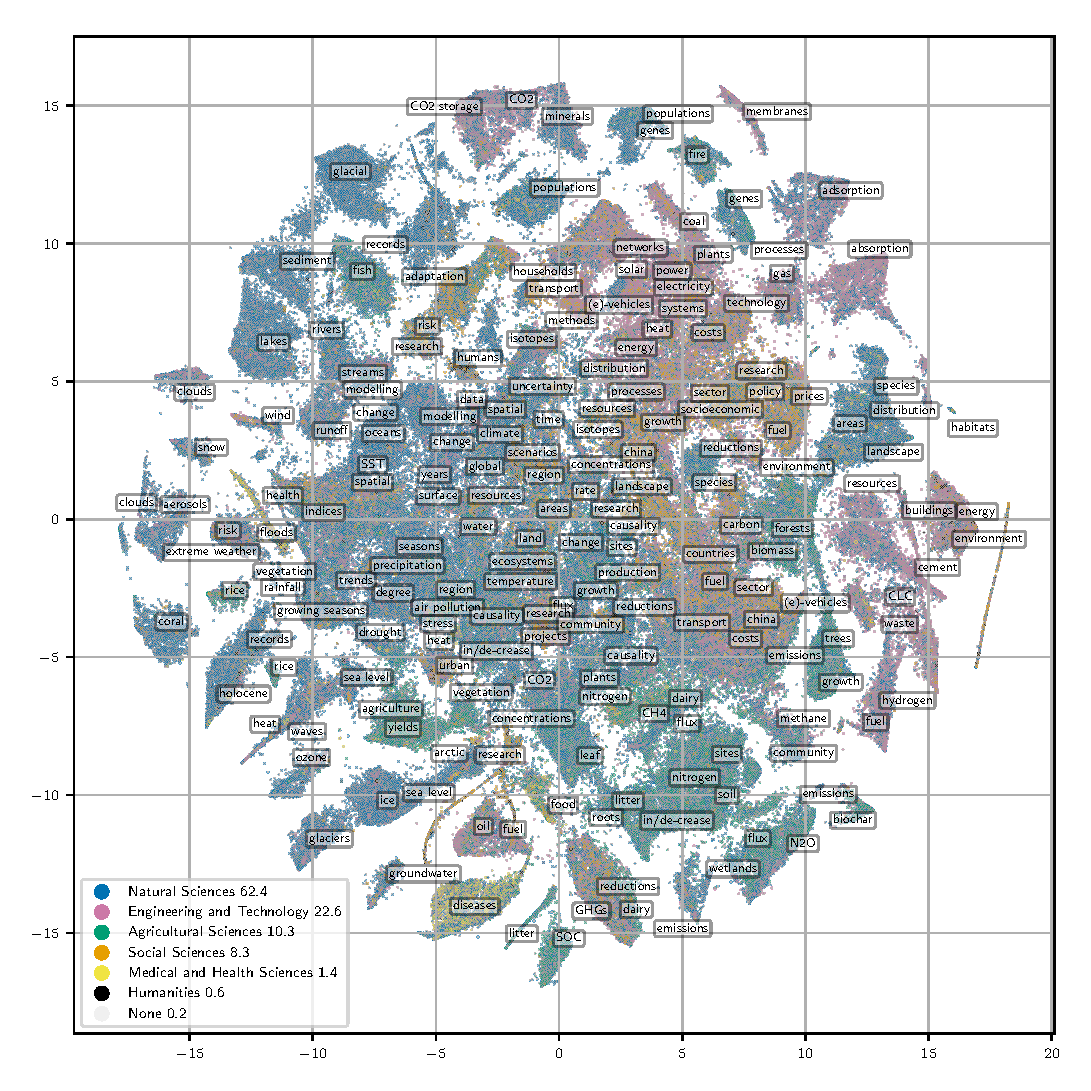
\includegraphics[width=180mm]{../plots_pub/all_topic_words_oecds.png}
				\caption{A map of the literature on climate change. Document positions are obtained by reducing the topic scores to two dimensions via t-SNE (see methods for further details). The two axes therefore have no direct interpretation, but represent a reduced version of similarities between documents across 140 topics. Documents are coloured by web of science discipline category. Topic labels are placed in the center of each of the large clusters of documents associated with each topic. }
				\label{oecd_topic_map}
			\end{center}
		\end{figure}
		
		
		
		Our map covers a broad range of topics, with related topics in clusters. Generally, topics related to climate science and impacts are on the left, while solution-oriented topics are on the right. More fine-grained research areas can also be distinguished. For example, publications related to urban infrastructure (\textbf{buildings}, \textbf{cement}, \textbf{waste}) are located on the right, physical climate impacts (\textbf{sea-level}, \textbf{droughts}  or [crop] \textbf{yield}) are in the lower left and energy systems are in upper right. Larger groups of documents at the fringes of the map relate mainly to one or two specific topics like \textbf{biochar} or \textbf{coral}. Interestingly, scenarios feature centrally in the map, at the interface between different scientific communities. This corresponds to their integrative nature in IPCC reports \cite{Moss2010}. %This map of the thematic structure of the literature could be useful for individual scientific communities or for climate change assessments.
		
		
		The disciplinary composition of this research topography indicated by the different colours in Figure \ref{oecd_topic_map} highlights the dominance of natural sciences in climate change research. More than 60\% of the literature is published in natural science journals. Similarly, 115 of 140 topics contain a greater share of publications from natural science journals than any other discipline. We calculate disciplinary entropy of topics as a measure of their degree of interdisciplinarity (Figure \ref{dis-entropy} and methods for details). This shows how research on \textbf{health}, \textbf{food}, or \textbf{policy} comes from a range of disciplines, while research on \textbf{ice} or \textbf{oceans} comes almost exclusively from the natural sciences). 
		
		
		\begin{figure}
			\begin{center}
				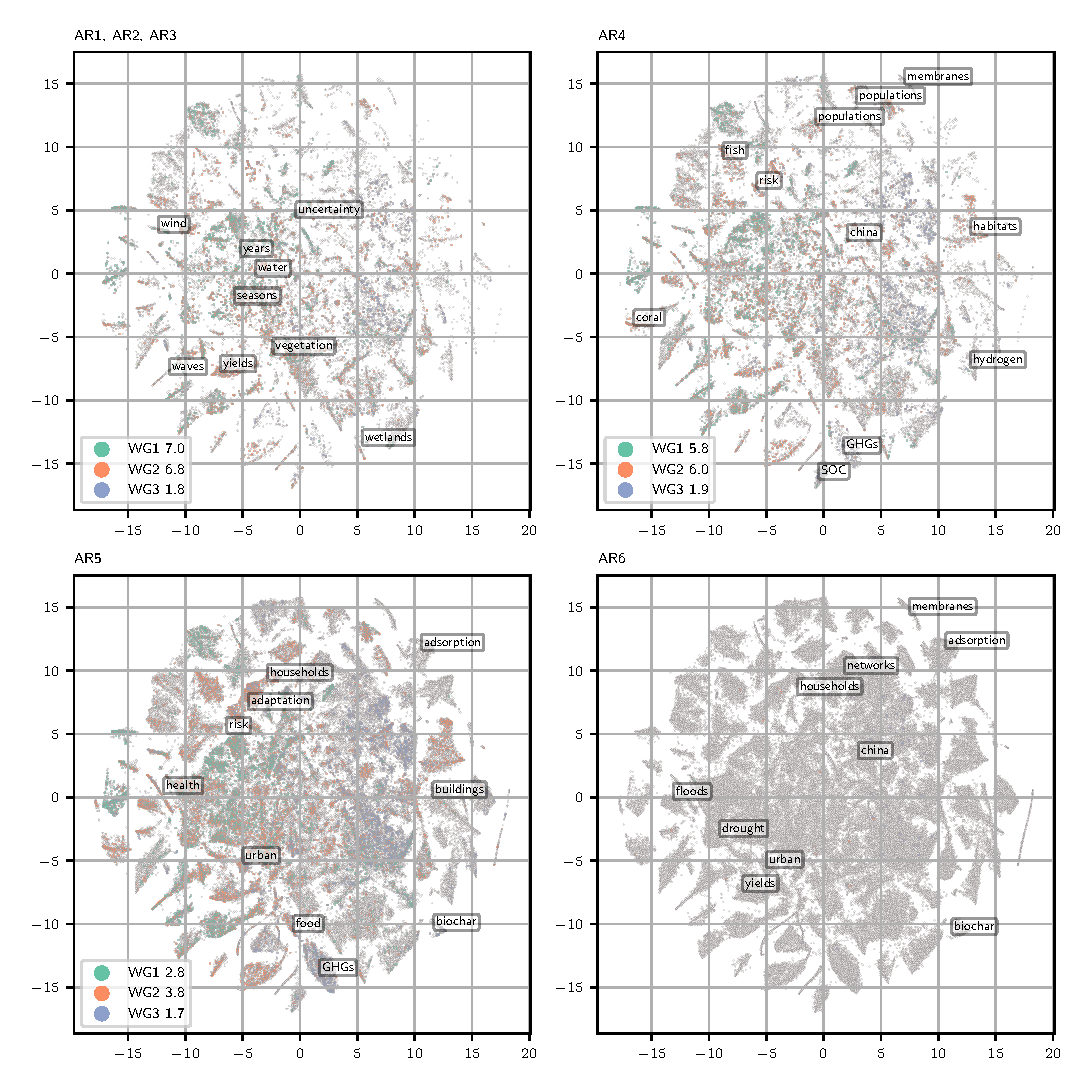
\includegraphics[width=180mm]{../plots_pub/topic_evolution_4.png}
				\caption{Evolution of the landscape of climate change literature. In each period, the 10 fastest growing topics are labelled. Where documents could be matched to IPCC citations, they are coloured by the working group citing them.}
				\label{evolution-map}
			\end{center}
		\end{figure}
		
		Finally, the topography shows the thematic evolution of the literature (Figure \ref{evolution-map}), with topics exhibiting distinct patterns of growth. Fast-growing topics in the last three assessment periods have included, among others, \textbf{coral}, \textbf{risks}, \textbf{adaptation}, \textbf{hydrogen}, \textbf{buildings}, \textbf{CO2 removal}, \textbf{networks} and \textbf{biochar}. \textbf{Biochar} is particularly remarkable in that the sizeable literature which emerged in AR5 was completely absent from the climate change literature beforehand. 
		The identification of new topics as they emerge, particularly as these are identified without prior knowledge of the literature, can help researchers and assessment-makers to keep abreast of a quickly evolving field.
		
		
		\subsection*{Research representation in IPCC reports}
		We apply our topic map to understand how IPCC assessments represent the science and respond to policymakers' and consulted experts' demands for more solution-oriented knowledge \cite{Kowarsch2017}.  Several studies have identified, made, or repeated claims of a disciplinary bias of IPCC assessments towards the natural sciences, and within the social sciences towards economics \cite{Bjurström2011, Victor2015, Hulme2010, Corbera2016}. Where these claims were based on an analysis of IPCC citations \cite{Bjurström2011}, they assess this without measurable baseline. 
		In view of the organisation's mandate to provide ``comprehensive, objective, open and transparent'' assessments of the available science \cite{IPCC2013}, our dataset of publications allows us - albeit imperfectly, as discussed in the concluding section - to study representation with a meaningful baseline. Further we provide an update to the last quantitative assessment of IPCC citations \cite{Bjurström2011}, which looked only at AR3. 
		This baseline forms a starting point for informed discussion about how to represent the literature according to the IPCC's priorities.  
		
		
		By matching the documents in our dataset to a set of references scraped from all published IPCC reports \cite{Minx2017l}, we assess the representation of a group of studies by comparing its share in IPCC citations with its share in the dataset of WoS studies on climate change (see methods). 		
		Figure \ref{oecd_rep}.a shows that social science documents (as identified by WoS) were indeed under-represented in AR3, but by AR5 were the most over-represented discipline, with a share in the literature cited by IPCC reports 1.32 times higher than their share in our WoS dataset. Likewise, social \& economic geography, political science, and "Other social sciences" were better represented in AR5 than economics. 	
		This challenges what we think we know about the IPCC. 
		Instead of under-representing the social sciences, the IPCC has been under-representing the Agricultural Sciences and Engineering \& Technology.
		%Humanities are also under-represented, although they make up a very small proportion of the total literature.
		
		
		The topography allows us to delve deeper into subjects that receive more or less attention in the IPCC. 
		%Figures \ref{oecd_rep}b and \ref{oecd_rep}c plot topic representation. 
		Figure \ref{oecd_rep}c shows that topics more commonly cited by IPCC working group I (WGI) are older and largely better represented in IPCC reports. These topics, for example \textbf{ozone}, \textbf{oceans}, and \textbf{aerosols}, are core topics for WGI, which addresses the physical science of climate change.
		
		The topics in the lower right of the graph are the most pertinent to the question of whether the IPCC is well representing knowledge on climate change. They are newer and until now have been under-represented in IPCC reports. Their novelty may be highly salient in a periodic assessment process. These topics are primarily in working group III, on mitigation and are ``solutions-relevant''. But while policymakers' demands for solutions-oriented IPCC assessments were often focussed on policy options, these under-represented new topics deal with more technical solutions and are found in technical disciplines within engineering \& technology and the agricultural sciences.
		
		Further, WGIII topics that are well represented contain a greater proportion of social science research (figure \ref{oecd_rep}b). The topics \textbf{countries}, \textbf{policy}, and \textbf{prices} are close to a proportional representation and are made up of around 30\% social science research. \textbf{Waste}, \textbf{biochar}, and \textbf{cement}, are more than 3 times more prevalent in the wider literature than in the literature cited by the IPCC, and are made up of around 5\% social science research. This pattern is not visible in other working groups (Figure \ref{socsci-wgs}).
		
		The difference between under-represented new topics and new topics that are better represented is intriguing. This is visible in figure \ref{evolution-map}, where in AR5, the clusters of documents around the, \textbf{buildings} and \textbf{biochar} topics contain few IPCC citations, whereas the clusters around, \textbf{adaptation} and \textbf{food} contain more. As shown in figure \ref{oecd_rep}c, \textbf{buildings} and \textbf{biochar} are 3.34 and 3.61 times more prevalent in the literature than in IPCC citations, while \textbf{food} is 1.22 times more prevalent in the literature and \textbf{adaptation} is 2.22 times more prevalent in IPCC citations respectively. %The IPCC, has been better at integrating new knowledge from these topics, and in general better at integrating new knowledge from WGII than WGIII topics.
		

		

		
		\begin{figure}[htp]
			\begin{center}
				\includegraphics[width=180mm]{../plots_pub/big_panel_representation.pdf}
				\caption{Representation in IPCC reports: \textbf{a)} by discipline, \textbf{b)} by social science proportion of WGIII topics, \textbf{c)} and novelty of all topics, where topics in the highest and lowest 10\% of either axis are labelled. Topics are coloured according to the working group from which they receive the most citations, although infrequently cited topics may not correspond to the relevant working group (see methods). Representation is the share of the subset of documents being cited by the IPCC divided by the share of the subset in the whole literature. We plot on a log scale so that 0.5 is equally distant to 1 as 2; plot labels show real values. Assessment period occurrence refers to the center of a topic's distribution across assessment periods (see methods for further details).}
				\label{oecd_rep}
			\end{center}
		\end{figure}
		
		
		\subsection*{Machine-learning for climate change assessments}
		
		

		Notwithstanding the over-representation of social science and under-representation of technical solutions in the IPCC with respect to the WoS, a
		 perfectly proportional representation of the literature is of course not optimal. A recommendation that the IPCC cite more or less of any part of the literature is by no means the goal of such an analysis. The IPCC, as a community of scientific experts, is vastly better placed to decide what is relevant than any algorithm. 
		As with many machine learning applications, we should be mindful of David Hume's is-ought problem. 
		Machine learning can help us to more efficiently understand and describe the landscape of climate change literature, but cannot tell us how things should be. 
		The results represent new knowledge about the interaction between the IPCC and the literature, which can have a variety of implications. 
		If the IPCC needs to include more social science knowledge \cite{Victor2015}, our analysis suggests that this is a result of insufficient production or funding of social science research on climate, rather than IPCC bias. 
		The under-representation of solutions-relevant topics (despite calls for solutions-oriented assessments), and the small proportion of social science research within these topics,  suggests areas for future highly relevant social science research, as well as opportunities for particularly fruitful interdisciplinary collaboration. 
		
		
		As a guide for future assessments, the map could facilitate well informed decisions about the representation of different areas of climate literature, from the early scoping process, through to selection by authors of individual studies.
		One advantage of topic modelling is that outcomes are not determined by any categorisation scheme imposed by the modeller, facilitating the discovery of ``unsearched'' for topics. 
		Highlighting recent research on, for example, membranes, biochar or e-vehicles, could prompt discussion in the scoping process about their inclusion in chapter outlines.
		This mode of discovery can act as a complement to human expertise, which may be better at identifying under-researched niches, existing biases or knowledge requirements.
		The methods shown here could also aid other processes in the production of IPCC reports, such as the identification of potential authors to achieve a better balance across sectors, regions and genders \cite{Corbera2016}. The possible benefits or risks of using data science methods for IPCC processes constitutes an important area for future research.
		Outside of the IPCC, this approach is part of ongoing attempts to make use of machine learning within evidence synthesis. This topographic map is a new approach to rapidly mapping very large literatures. 
		
		Our dataset of more than 400,000 publications represents a wealth of knowledge on climate change and climate solutions, but is by no means exhaustive. We repeat an established query \cite{Haunschild2016}, granting that it may have imperfections. Furthermore, we miss publications not in WoS  (some small journals, some books, and most grey literature, not to mention indigenous knowledge \cite{Ford2016b}); and studies relevant for the work of the IPCC, that do not directly mention climate change (for example on energy policy). We argue that this remains a reasonable system boundary given data availability, and stress that documents not included in our study alter our findings only if they have systematically different patterns of citation by the IPCC. 
		A future topography could be improved by making use of more sources of climate change knowledge, extracting and classifying information from full texts, or exploring author networks and interdisciplinarity. 
		Most importantly, exploring machine learning applications that support IPCC authors in their assessments would prepare the IPCC for the age of big literature.
		
		
	\end{linenumbers}
	
	\appendix
	
	%\listoffigures
	\linespread{1}
	\bibliography{Mendeley}
	
	\bibliographystyle{unsrt}
	
	%	\documentclass{article}
\usepackage[a4paper, total={6in, 8in}]{geometry}
\usepackage{graphicx}
\usepackage{url}
\usepackage{natbib}
\usepackage{todonotes}
\usepackage{booktabs}
\usepackage{lineno}
\usepackage{color}
%\usepackage{auto-pst-pdf}
\usepackage[colaction]{multicol}
\usepackage{caption}
\usepackage{svg}
\usepackage{authblk}
\usepackage{standalone}
\usepackage[section]{placeins}

\makeatletter
\renewcommand{\maketitle}{\bgroup\setlength{\parindent}{0pt}
	\begin{flushleft}
		
		{\huge\textbf{\@title}}
		
		\bigskip
		
		{\large\textbf{\@author}}
		
		\bigskip
		
		{\large{Draft current \@date}}
		
	\end{flushleft}\egroup
}
\makeatother


\begin{document}
	% Title
	\title{A Topic Model of Climate Change Literature}
	\title{Words, words, words: Mapping the Matter of Climate Change Literature}
	\title{A Topography of Climate Change Research - Methods}
	\author[1,2]{Max Callaghan}
	
	\affil[1]{Mercator Research Institute on Global Commons and Climate Change, Torgauer Straße, 10829 Berlin, Germany}
	\affil[2]{School of Earth and Environment, University of Leeds, Leeds LS2 9JT, United Kingdom}
	\maketitle
	\begin{linenumbers}
	
	\setcounter{figure}{0}
	\renewcommand\thefigure{SI.\arabic{figure}}  
		
	\subsection*{Data}
	
	This study reproduces the query developed by \citep{Grieneisen2011}, which is carried out on the Web of Science core collection. Though not exhaustive, the Web of Science gives a good coverage of the literature in major peer-reviewed journals.	Each document is assigned to an assessment period according to the timeline shown in table 1.
	
	We use the references scraped from IPCC assessment reports from \citep{Minx2017l}, and attempt to match these with the results from the web of science. Table \todo{}[x] shows the percentage of IPCC citations matched in each working group for each assessment report.
		
	\subsection*{Pre-processing}
	
	Data quality in earlier Web of Science results is poorer, and some documents have missing abstracts. In the quantification of the size of the literature and its vocabulary in table [], titles are substituted for abstracts where they are not available.  The words of the documents are lemmatized/stemmed, replacing different forms of the same word (i.e. word/words) with a single instance. Commonly occuring words, or ``stopwords'' are removed, as are all words shorter than 3 characters, and all words containing only punctuation or numbers.
	
	The documents are transformed into a document-term matrix, where each row represents a document, and each column represents a unique word.  Each cell contains the number of that column's terms in that document. Only terms which occur more than once are considered.
	
	For the calculation of the topic model, documents with missing abstracts are ignored, and the document term matrix is transformed into a document
	frequency-inverse document frequency (tf-idf) matrix, where scores are scaled according to the frequency of their occurence in the corpus. This gives more weight to terms which appear in few documents, and less weight to those which appear in many.
	
	\begin{equation}
	tf(t,d) = f_{t,d} \mathrm{,}\quad idf(t,D) = \log\frac{N}{|\{d \in D:t \in d\}|}
	\end{equation} 
	
	\subsection*{Topic Model}
	
	We use non-negative Matrix Factorisation (NMF) \cite{Lee1999}, an approach to topic modelling which factorises the term-frequency-inverse document frequency matrix \( V \) into the matrices \(W\), the topic-term matrix, and \( H \) the document-topic matrix, whose product approximates \(V\):
	
	\begin{equation}
		V_{i\mu} \approx (WH)_{i\mu} = \sum_{a=1}^{r}W_{ia}H_{a\mu}
	\end{equation}
	
	As demonstrated in Figure \ref{doc-topic}, each topic is represented as a set of word scores, and each document a set of topic scores. The combination of the two give the word scores in the document. For clarity in the figure, these are shown as simple counts, but in the model these are scaled according to each term's frequency within the corpus as explained above.
	
	Topics are calculated using the scikitlearn library \cite{Pedregosa2011}, and are saved in a database and topic visualisation system based on \cite{Chaney2012} \footnote{The system adds new functionality to \cite{Chaney2012} and combines it with a system for managing sets of documents and queries. The code and additional information is published online at \url{https://github.com/mcallaghan/tmv}}. 	
	
	\subsubsection*{Model selection}
	
	Topic models are calculated for 70, 80, 90, 100, 110, 120, 130 and 140 topics. The relative usefulness of each model was assessed subjectively by the authors, based on inspection of the online visualisation tool, and the spreadsheet \textbf{topic\_comparison.xlsx} accompanying the supporting information. The spreadsheet shows each set of topics in adjacent columns. Topics from each model are placed next to the topics with the largest number of each topic's 10 highest scoring words in common. This helps authors to find an appropriate level of granularity for the analysis. 
			
	\subsubsection*{Topic Representation and Newness}
	
	To calculate topic representation in IPCC reports we divide each topic's share in the subsample of documents cited by IPCC reports by its share in the whole corpus. 
	
	We calculate a topic's total score as the sum of document-topic scores. A topic's window score is the sum of document-topic scores considering only documents in the given time window. To represent a topic's newness, we multiply each assessment period number by the share of it's total score occurring in that window, and take the mean of these scores. A topic in which 100\% of documents which make it up occurred in assessment period 1 (6) would thereby receive a score of 1 (6), while a topic evenly distributed across all assessment periods would receive a score of 3.5.
	
	
	\subsubsection*{Disciplinary Entropy}
	
	Disciplinary Entropy inverts the measurement of a conference's topical diversity suggested in \cite{Hall2008}, by measuring a topic \(z\)'s entropy \(H\), where 
	
	\begin{equation}
		H(f|z) = -\sum_{i=1}^K \hat{p}(f|z) \log \hat{p}(f|z) 
	\end{equation}
	
	based on the empirical distribution of a field \(f\) in the documents \(d\) in each topic:
	
	\begin{equation}
		\hat{p}(f|z) = \sum_{d:z_d=z} \hat{p} (f|d) \hat{p} (d|z)
	\end{equation}

	\begin{figure}
		\begin{center}
			\includegraphics[width=1\linewidth]{plots_pub/topic_oecd_entropy.pdf}
			\caption{SI Disciplinary Entropy}
			\label{dis-entropy}
		\end{center}
	\end{figure}	
	
	
	
	\begin{figure}
		\begin{center}
			\includegraphics[width=1\linewidth]{plots_pub/single_doc_3_536594_1861.pdf}
			\caption{SI Topic make up of a single document}
			\label{doc-topic}
		\end{center}
	\end{figure}

	\begin{figure}
	\begin{center}
		\includegraphics[width=1\linewidth]{plots_pub/ipcc_rep_wcs_simplified.pdf}
		\caption{SI Representation by subfield}
		\label{subfield}
	\end{center}
\end{figure}

\begin{figure}
	\begin{center}
		\includegraphics[width=1\linewidth]{plots_pub/wgs_socsci.pdf}
		\caption{SI Social science \& representation in topics across working groups}
		\label{socsci-wgs}
	\end{center}
\end{figure}

\subsection*{Glossary}


\noindent\textbf{ncep:} National Centers for Environmental Protection

\noindent\textbf{fco:} Fugacity of Carbon Dioxide

\noindent\textbf{pfc:} Perflourocompound

\noindent\textbf{otcs:} Open Top Chambers

\noindent\textbf{dtr:} Diurnal Temperature Range

\noindent\textbf{sres:} Special Report on Emissions Scenarios (200)

\noindent\textbf{petm:} Paleocene Eocene Thermal Maximum

\noindent\textbf{amf:}  Arbuscular Mycorrhizal Fungal

\noindent\textbf{sf5cf3:} trifluoromethyl sulfur pentafluoride (A Potent Greenhouse Gas Identified in the Atmosphere, 2000)

\noindent\textbf{clc:} Chemical Looping Combustion

\noindent\textbf{cwd:} Coarse woody debris

\noindent\textbf{etm:} Enhanced Thematic Mapper (NASA satellite sensor)

\noindent\textbf{cmip5:} Coupled Model Intercomparison Project 5 (Starting 2008)

\noindent\textbf{cmip3:} Coupled Model Intercomparison Project phase 3 (first published 2007 \cite{Meehl2007})

\noindent\textbf{mofs:} metal-organic frameworks (for CO2 storage)

\noindent\textbf{sdm:} statistical-dynamical model

\noindent\textbf{mmms:} Mixed Matrix Membranes (for CO2 capture)

\noindent\textbf{cop21:} 21st Conference of Parties (Paris 2015) 

\noindent\textbf{c3n4:} Carbon nitride (a synthetic nanomaterial used for hydrogen production)

\noindent\textbf{sdg:} Sustainable Development Goals

\noindent\textbf{indc:} Intended Nationally Determined Contributions

		
	\end{linenumbers}

\linespread{1}
%\bibliography{Mendeley}

\begin{thebibliography}{1}
	
	\bibitem{Grieneisen2011}
	Michael Grieneisen and Minghua Zhang.
	\newblock {The Current Status of Climate Change Research}.
	\newblock {\em Nature Climate Change}, 1:72--73, 2011.
	
	\bibitem{Minx2017l}
	Jan~C. Minx, Max Callaghan, William~F. Lamb, Jennifer Garard, and Ottmar
	Edenhofer.
	\newblock {Learning about climate change solutions in the IPCC and beyond}.
	\newblock {\em Environmental Science {\&} Policy}, 2017.
	
	\bibitem{Lee1999}
	D~D Lee and H~S Seung.
	\newblock {Learning the parts of objects by non-negative matrix factorization.}
	\newblock {\em Nature}, 401(6755):788--91, 1999.
	
	\bibitem{Pedregosa2011}
	Fabian Pedregosa, Ga{\"{e}}l Varoquaux, Alexandre Gramfort, Vincent Michel,
	Bertrand Thirion, Olivier Grisel, Mathieu Blondel, Peter Prettenhofer, Ron
	Weiss, Vincent Dubourg, Jake Vanderplas, Alexandre Passos, David Cournapeau,
	Matthieu Brucher, Mattheiu Perrot, and {\'{E}}douard Duchesnay.
	\newblock {Scikit-learn: Machine Learning in Python Fabian}.
	\newblock {\em Journal of Machine Learning Research}, 12:2825--2830, 2011.
	
	\bibitem{Chaney2012}
	Allison J~B Chaney and David~M. Blei.
	\newblock {Visualizing Topic Models}.
	\newblock {\em Icwsm}, pages 419--422, 2012.
	
	\bibitem{Hall2008}
	David Hall, Daniel Jurafsky, and Christopher~D. Manning.
	\newblock {Studying the history of ideas using topic models}.
	\newblock {\em Proceedings of the Conference on Empirical Methods in Natural
		Language Processing - EMNLP '08}, pages 363--371, 2008.
	
	\bibitem{Meehl2007}
	Gerald~A. Meehl, Curt Covey, Thomas Delworth, Mojib Latif, Bryant McAvaney,
	John~F.B. Mitchell, Ronald~J. Stouffer, and Karl~E. Taylor.
	\newblock {The WCRP CMIP3 multimodel dataset: A new era in climatic change
		research}.
	\newblock {\em Bulletin of the American Meteorological Society},
	88(9):1383--1394, 2007.
	
\end{thebibliography}


\bibliographystyle{unsrt}

\end{document}
	
\end{document}